\documentclass[a4paper, 12pt]{article}
\usepackage[slovene]{babel}
\usepackage[utf8]{inputenc}
\usepackage[T1]{fontenc}
\setlength{\parindent}{0px}
\setlength{\parskip}{10px}
%standard

\usepackage{listings}
\usepackage{color}
\usepackage{amssymb}
\usepackage{tikz}
\usepackage{pgfplots}

\title{Avditorne vaje za Programiranje II}
\author{Matej Blagšič}

\begin{document}
%-----------------------------


\definecolor{dkgreen}{rgb}{0,0.6,0}
\definecolor{gray}{rgb}{0.5,0.5,0.5}
\definecolor{mauve}{rgb}{0.58,0,0.82}
\definecolor{lgray}{RGB}{250,250,250}
	\lstset{
		frame=l,%single
		language=C,
		aboveskip=3mm,
		belowskip=3mm,
		showstringspaces=false,
		columns=flexible,
		basicstyle={\small\ttfamily},
		numbers=none,
		numberstyle=\tiny\color{gray},
		keywordstyle=\color{blue},
		commentstyle=\color{dkgreen},
		stringstyle=\color{mauve},
		breaklines=true,
		breakatwhitespace=true,
		tabsize=4,
		backgroundcolor=\color{lgray},
		moredelim=**[is][\color{dkgreen}]{@}{@}
	}
%--------------------------------
	
	
	\maketitle
	\thispagestyle{empty}
	\pagebreak
	\setcounter{page}{1}
	\tableofcontents
	\pagebreak
%-----------------------------------Tu naprej

\section{Prva vaja}

\section{Druga vaja}
\subsection*{Prva naloga:}

\underline{Izračunaj $\int_{x0}^{x1}2x^2-5x dx$. Rezultat preveri analitično.}	\

Če analitično integriramo itegral, dobimo: $\int_{x0}^{x1}2x^2-5x dx = 2\frac{x1^3}3-5\frac{x0^2}2$\

Sedaj spišimo kodo:
\begin{lstlisting}
int main(){
	float x, x0, x1;
	float dx = 0.0000001;
	float integral = 0;
	printf("vnesi spodno mejo");
	scanf("%f",&x0);
	printf("Vnesi zgornjo mejo");
	scanf("%f",&x1);

	for(x=x0; x<x1;x+=dx){
		integral += dx*(2*x*x-5*x);
	}

	printf("Integral znasa: %f\n", integral);
	return 0;
}
\end{lstlisting}
Pri programu nam spremenljivka dx sporoči, kako širok del območja integrira. Manjša, kot je cifra, bolj natančno izračuna. x0 in x1 sta spodnja in zgornja meja integracije, x pa je spremenjivka, ki jo premikamo po intervalu za dx razdaljo in seštevamo pravokotnike.
	

*TOLE JE TEST ZA GRAF INTEGRALA*
\begin{tikzpicture}
\begin{axis}
\addplot[color=red]{x^2};
\end{axis}
\end{tikzpicture}
%Here ends the furst plot
\hskip 5pt
%Here begins the 3d plot
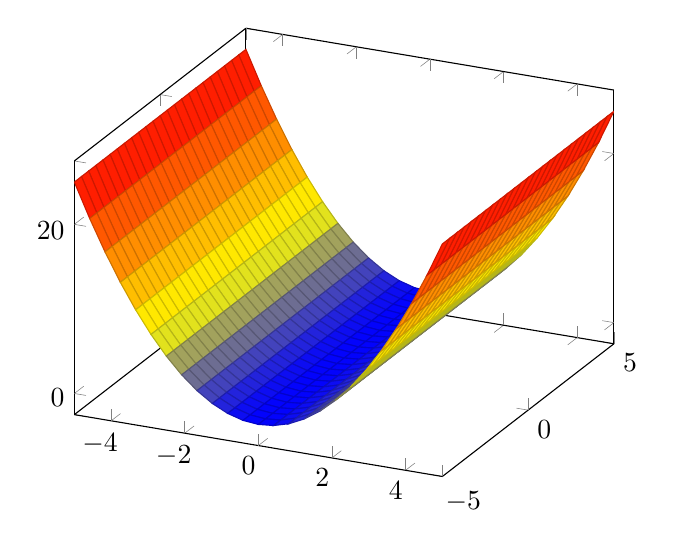
\begin{tikzpicture}
\begin{axis}
\addplot3[
surf,
]
{x^2};
\end{axis}
\end{tikzpicture}


	
	
	
	
	
	
	
	
\end{document}